% Capítulo de ejemplo para colocar descripción del problema
\chapter{Marco Teórico}

\section{Computación neuromórfica}

La computación neuromórfica surge como un paradigma de cómputo inspirado en la organización y el funcionamiento del cerebro, con el objetivo de desarrollar sistemas de inteligencia artificial que, además de precisos, sean eficientes en términos de energía, latencia y escalabilidad física \cite{malcolm2023comprehensivereviewspikingneural, Choi2025}. A diferencia de los enfoques de aprendizaje profundo convencionales, cuyo procesamiento suele depender de operaciones continuas e intensivas, como multiplicaciones matriciales, este paradigma organiza el cómputo alrededor de eventos discretos y de arquitecturas dispersas \cite{Yao2024neuromorphicchip, yan2026reconsideringenergyefficiencyspiking}. En particular, estos eventos pueden corresponder a espigas neuronales, señales breves que comunican actividad entre neuronas y que permiten activar el procesamiento solo cuando existe información relevante \cite{Wunderlich2021EventProp}.

Mientras que las redes profundas tradicionales pueden requerir hardware de alto consumo energético para tareas de reconocimiento complejas, el cerebro humano realiza múltiples funciones cognitivas con un presupuesto energético aproximado de 20 W \cite{Clarke1999}. Esta diferencia ha impulsado la búsqueda de alternativas inspiradas en la biología \cite{doi:10.1073/pnas.1604850113efficientneuromorphic, Henkes2024snnnonlinearregression}. La computación neuromórfica busca aproximarse a esta eficiencia mediante arquitecturas que modelan neuronas, sinapsis y comunicación mediante espigas, aprovechando la dispersión temporal de la actividad neuronal \cite{Kudithipudi2025Neuromorphiccomputingatscale, Choi2025}. De este modo, el cómputo puede ejecutarse de manera dirigida por eventos (event-driven), reduciendo operaciones redundantes durante intervalos sin actividad neuronal \cite{Yao2024neuromorphicchip}.

Las redes neuronales de espigas (Spiking Neural Networks, SNN) constituyen uno de los modelos computacionales centrales de la computación neuromórfica y suelen considerarse la tercera generación de redes neuronales artificiales (Artificial Neural Networks, ANN) \cite{MAASS19971659ssnthirdgeneration}. En estas redes, la información se representa mediante trenes de espigas, por lo que el tiempo pasa a ser una variable explícita del procesamiento, a diferencia de las redes de segunda generación basadas principalmente en activaciones continuas \cite{Henkes2024snnnonlinearregression}. Una neurona integra las señales de entrada y, cuando su estado supera un umbral, emite una espiga, reinicia o actualiza su estado interno y continúa su evolución temporal \cite{Izhikevich2003}. Así, una SNN puede codificar información tanto en la cantidad de espigas como en sus instantes de ocurrencia, lo que resulta apropiado para procesar secuencias, series temporales y problemas donde la latencia de respuesta es relevante \cite{Zanatta2024snnrlrobotic, Voudaskas2025snninimaging, Ding2025neuroparadigms}.

Una característica central de las SNN es que su dinámica se modela mediante ecuaciones diferenciales o reglas discretas de integración temporal \cite{Izhikevich2003}, lo que permite representar fenómenos como adaptación, disparo repetitivo y ráfagas de actividad con modelos relativamente compactos \cite{Izhikevich2003}. En comparación con otros modelos neuronales biológicamente plausibles, las SNN ofrecen una relación favorable entre fidelidad biológica y costo computacional \cite{Schuman2022Opportunities}, lo que explica su uso en simulación de grandes poblaciones neuronales.

La vinculación entre SNN y hardware neuromórfico es estrecha, porque las arquitecturas neuromórficas suelen estar diseñadas precisamente para ejecutar redes de espigas de manera eficiente \cite{Schuman2022Opportunities, Muir2025commercialsuccessforneuromorphictechnologies, Yao2024neuromorphicchip}. Diversos desarrollos recientes han mostrado plataformas con consumos muy bajos, y en general la literatura coincide en que el potencial de las SNN es mayor en entornos donde la eficiencia energética y la ejecución en tiempo real son requisitos críticos \cite{yan2026reconsideringenergyefficiencyspiking}. Por eso, la computación neuromórfica no debe entenderse solo como una idea de inspiración biológica, sino como una línea concreta de diseño de sistemas inteligentes \cite{Kudithipudi2025Neuromorphiccomputingatscale}.

Sin embargo, las SNN presentan un desafío importante: su entrenamiento es más difícil que el de las redes convencionales, esto debido a que las funciones de disparo son no diferenciables, lo que impide aplicar directamente Backpropagation en su forma estándar \cite{10.3389/fnins.2024.1383844directtrainingsnn}. Por ello, se han propuesto alternativas como gradientes surrogados, STDP, conversión ANN-SNN y neuroevolución, cada una con distintos compromisos entre precisión, costo y plausibilidad biológica \cite{Schuman2022Opportunities}.

En el contexto de esta tesis, las SNN constituyen la base conceptual sobre la cual se plantea el problema de optimización. La idea no es solo entrenar una red para que clasifique bien, sino hacerlo manteniendo una estructura esparsa y eficiente \cite{malcolm2023comprehensivereviewspikingneural}, coherente con el espíritu de la computación neuromórfica. Por eso, la combinación entre SNN, optimización evolutiva y esparsidad estructural se ajusta naturalmente al problema estudiado.

%-----------------------------

\section{Redes neuronales de espigas (SNN)}

Un modelo formal típico de SNN se describe como un grafo dirigido $G = (V, E)$, donde cada nodo $i \in V$ representa una neurona y cada arista $(j,i) \in E$ representa una sinapsis desde la neurona presináptica $j$ hacia la neurona postsináptica $i$ \cite{Hwang2020snnmembranepotential, Yamazaki2022snnapplications}. Cada sinapsis está asociada a un peso sináptico $w_{ij}$ \cite{Sanaullah2023snnmathematicalmodels} que modula la contribución del potencial postsináptico excitatorio o inhibitorio (EPSP/IPSP) sobre la neurona postsináptica \cite{Hwang2020snnmembranepotential}.

La dinámica interna de cada neurona se modela mediante una o más variables de estado continuas en el tiempo, siendo la principal el potencial de membrana $v_i(t)$, que integra las corrientes sinápticas entrantes y tiende a relajarse hacia un potencial de reposo debido a una fuga \cite{Fontaine2014spiketresholdmembrane}. 

% En modelos de tipo leaky integrate‑and‑fire (LIF) \cite{Gerstner2002spikingneuronmodels}, la dinámica subumbral del potencial de membrana se modela habitualmente mediante una ecuación diferencial de primer orden del tipo

% \begin{equation}
%     \tau_m\dfrac{dv_i(t)}{dt}=-\left(v_i(t)-v_{rest}\right)+RI(t)
% \end{equation}

% donde $\tau_m$ es la constante de tiempo de membrana, $v_{rest}$ es el potencial de reposo, $R$ es la resistencia de membrana e $I(t)$ representa la corriente sináptica total que recibe la neurona $i$ \cite{Gerstner2002spikingneuronmodels}. La corriente sináptica total suele expresarse como la suma ponderada de contribuciones provenientes de todos los spikes presinápticos, pudiendo desplazar el potencial de membrana por encima o por debajo del potencial de reposo \cite{Hwang2020snnmembranepotential, Fontaine2014spiketresholdmembrane}.

El procesamiento discreto de la información en una SNN se produce cuando el potencial de membrana \(v_i(t)\) alcanza un umbral de disparo \(v_{\text{th}}\). En ese instante, la neurona \(i\) emite una espiga y genera un evento de salida en el tiempo \(t\), el cual puede propagarse hacia las neuronas postsinápticas. Posteriormente, su estado se reinicia de acuerdo con las ecuaciones del modelo neuronal utilizado, permitiendo que la neurona continúe integrando nuevas entradas y pueda emitir futuras espigas \cite{Izhikevich2003}.

%-------------------------------------------------

\section{Modelo neuronal Izhikevich}\label{sec:izhikevich}

El modelo de Izhikevich se formula como un sistema de dos ecuaciones diferenciales ordinarias acopladas para el potencial de membrana $v$ y una variable de recuperación $u$, más una regla de reinicio después del disparo \cite{Izhikevich2003}. La dinámica se describe mediante

\begin{equation}
    \dfrac{dv}{dt} = 0.04v^2+5v+140-u+I
\end{equation}

\begin{equation}
    \dfrac{du}{dt}=a(bv-u)
\end{equation}

donde $I$ representa la corriente sináptica o inyectada externa. 


Cuando el potencial de membrana alcanza el umbral de disparo, típicamente fijado en $v\geq30mV$, se aplica una condición de reinicio del tipo $v \leftarrow c$ y $u \leftarrow u+d$, que modela el comportamiento posterior al spike. La no linealidad cuadrática $0.04v^2$ es suficiente para capturar la iniciación del potencial de acción y hace que el modelo sea canónicamente equivalente a una amplia clase de modelos biológicamente detallados tipo Hodgkin-Huxley, a través de un cambio de coordenadas. Los patrones de disparo reproducibles por estas ecuaciones diferenciales se pueden observar en la Figura \ref{fig:patrones_disparo_izhikevich}.

\begin{figure}
    \centering
    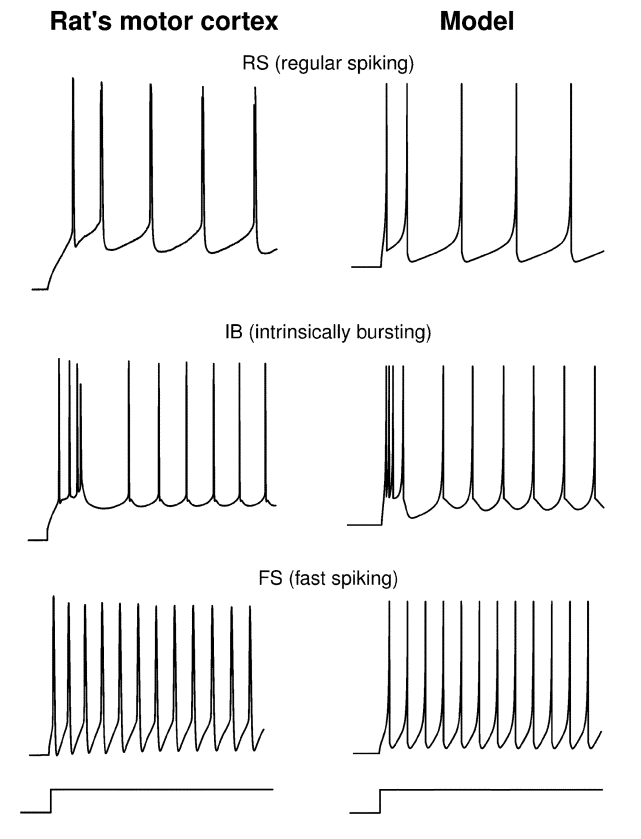
\includegraphics[width=0.5\linewidth]{images/patrones_disparo_izhikevich.png}
    \caption{Patrones de disparo del modelo neuronal Izhikevich. Extraído de Izhikevich \cite{Izhikevich2003}.}
    \label{fig:patrones_disparo_izhikevich}
\end{figure}

En el modelo, $v$ representa el potencial de membrana efectivo de la neurona y se escala en unidades comparables a milivoltios, con un potencial de reposo típico entre aproximadamente $-70$ y $-60 mV$ según el parámetro de acoplamiento \cite{Izhikevich2003}. La variable $u$ es una variable de recuperación que integra el efecto combinado de la activación de corrientes de potasio y de la inactivación de corrientes de sodio, proporcionando una realimentación negativa lenta sobre $v$. Esta variable $u$ permite capturar fenómenos como la adaptación de frecuencia, los pospotenciales hiperpolarizantes y ciertas oscilaciones subumbrales en un espacio de estados bidimensional, lo cual simplifica el análisis dinámico respecto de modelos de mayor dimensión.

El parámetro $a$ controla la escala temporal de la variable de recuperación $u$, de modo que valores pequeños de $a$ producen recuperaciones lentas y valores grandes generan dinámicas de recuperación más rápidas. El parámetro $b$ regula la sensibilidad de 
$u$ a las variaciones subumbrales del potencial de membrana $v$, y acoplamientos más fuertes pueden inducir oscilaciones subumbrales o disparo de umbral bajo. El parámetro $c$ fija el valor de reinicio del potencial de membrana después del disparo, representando el efecto de conductancias de potasio de alto umbral que llevan el potencial a niveles hiperpolarizados; un valor típico es $c\approx-65mV$ para neuronas de disparo regular. El parámetro $d$ determina el incremento de la variable de recuperación $u$ tras cada potencial de acción, lo que modela la acumulación de corrientes lentas y controla el grado de adaptación de frecuencia u otros regímenes dinámicos. Combinaciones específicas de $(a,b,c,d)$ permiten mapear distintos tipos de neuronas, lo que convierte a este modelo en un esquema parametrizable para múltiples fenotipos de disparo.

Mediante una elección adecuada de $(a,b,c,d)$, el modelo reproduce el disparo regular (\textit{regular spiking}, RS) característico de muchas neuronas piramidales. El modelo es capaz de producir muchos patrones de disparo que pueden ser usados en diferentes situaciones. Los diferentes modelos y comportamientos neuronales se pueden observar en las Figuras \ref{fig:patrones_disparo_izhikevich} y \ref{fig:disparos_izhikevich}.

\begin{figure}
    \centering
    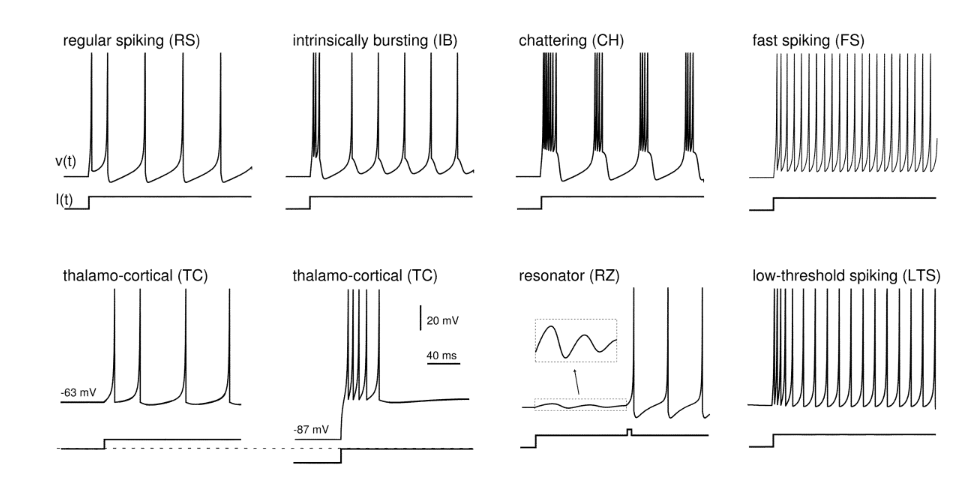
\includegraphics[width=1\linewidth]{images/disparos_izhikevich.png}
    \caption{Tipos de neuronas correspondiente a diferentes valores de a, b, c y d. Extraído de Izhikevich \cite{Izhikevich2003}.}
    \label{fig:disparos_izhikevich}
\end{figure}

La presente tesis adopta el modelo de Izhikevich porque ofrece un compromiso explícito entre plausibilidad biológica y eficiencia computacional, permitiendo simular redes de decenas de miles de neuronas en tiempo real con resolución del orden de milisegundos en hardware convencional. Esta eficiencia resulta especialmente adecuada para el escenario de optimización evolutiva multiobjetivo y esparsa a gran escala que se aborda en este trabajo, donde es necesario evaluar iterativamente un gran número de configuraciones de redes de disparo. Al mantener solo dos variables de estado continuas y una no linealidad cuadrática, el modelo facilita el estudio sistemático de patrones de disparo y regímenes de operación de SNN. Adicionalmente, el hecho de que el modelo sea canónico en el sentido de que puede derivarse de modelos de conductancias tipo Hodgkin–Huxley mediante reducciones apropiadas respalda su uso como representación compacta de neuronas biológicamente realistas en contextos de computación neuromórfica.

%--------------------------------

\section{Codificación y decodificación de spikes}\label{sec:codificacion-y-deco}

En una red neuronal de espigas, el codificador es el mecanismo que convierte datos continuos o discretos en trenes de espigas adecuados para su procesamiento temporal \cite{Wang2019spiketrainkernels, MAASS19971659ssnthirdgeneration}, mientras que el decodificador transforma estos trenes de espigas de salida en decisiones o valores numéricos interpretables \cite{Tavanaei2019dlinsnn, Schuman2022Opportunities}. Estos mecanismos son necesarios porque las SNN operan sobre eventos binarios en el tiempo \cite{Schuman2022Opportunities}, pudiendo aplicarse en la capa de entrada para transformar características como píxeles o variables sensoriales en espigas, mientras que la decodificación se emplea en la capa de salida para leer la clase o el valor estimado a partir de la actividad final \cite{Wang2019spiketrainkernels}.

\paragraph{Codificación Poisson (rate coding)} En el \textit{rate coding}, cada característica de entrada se representa mediante un tren de espigas cuya frecuencia media de disparo es proporcional al valor de la señal, de modo que entradas más grandes producen tasas de disparo más altas en una ventana temporal fija \cite{Guo2021neuronalcodingsnn}. Un modelo habitual para este tipo de codificación es el proceso de Poisson, en el que el número de espigas generadas en un intervalo de tiempo sigue una distribución de Poisson con parámetro $\lambda t$ que depende de la magnitud de la entrada \cite{Pachitariu2002modelsspiketrains, Yamazaki2022snnapplications}. En implementaciones prácticas de SNN, esta codificación Poisson suele aproximarse generando en cada paso de simulación una espiga con probabilidad proporcional al valor normalizado de la característica, lo que conduce a un tren de spikes estocástico cuya tasa de disparo coincide, en promedio, con la intensidad deseada \cite{Pachitariu2002modelsspiketrains}. Para decodificar bajo rate coding en tareas de clasificación, es común acumular el número de espigas de cada neurona de salida en una ventana de tiempo y seleccionar como clase predicha aquella neurona con mayor conteo de spikes \cite{Guo2021neuronalcodingsnn}.

\paragraph{Time‑to‑first‑spike (TTFS)}
En la codificación time‑to‑first‑spike (TTFS), la información se representa mediante la latencia del primer disparo: cada neurona de entrada emite a lo sumo una espiga y el tiempo hasta esa primera espiga codifica la intensidad del estímulo, de modo que valores más altos suelen corresponder a spikes más tempranos \cite{Guo2021neuronalcodingsnn, Bonilla2022ttfs}. Diversos trabajos teóricos y experimentales han mostrado que un código de latencia puede transmitir gran cantidad de información con muy pocas espigas, lo que permite decisiones muy rápidas y potencialmente un consumo energético reducido en hardware neuromórfico \cite{Bonilla2022ttfs}. En particular, estudios comparativos de esquemas de codificación en SNN profundas convertidas desde redes artificiales han demostrado que TTFS puede mayor exactitud de clasificación, con la menor latencia de inferencia y el número más bajo de operaciones sinápticas frente a rate coding y otros códigos temporales \cite{Guo2021neuronalcodingsnn}. La decodificación en redes TTFS suele basarse en reglas de “primero en disparar”, en las que la clase se asigna a la neurona de salida cuya espiga aparece con menor latencia dentro de una ventana de observación \cite{Bonilla2022ttfs, Goltz2021ttfsdeeplearning}.

\paragraph{Winner‑takes‑all (WTA)}
Winner‑takes‑all (WTA) es un principio de cómputo competitivo en el que un conjunto de neuronas recibe entradas similares y, a través de interacción selectiva, solo una neurona o un pequeño subconjunto queda finalmente activa, típicamente la que recibe el estímulo más fuerte \cite{Oster2009wtaspikes}. En redes de espigas, estos mecanismos WTA se han utilizado como bloques de decisión para categorización, selección de acciones y modelos atencionales, dado que permiten transformar un patrón complejo de actividad de población en una salida discreta fácilmente interpretable. En el contexto de decodificación en SNN, una regla WTA puede aplicarse tanto sobre el conteo de espigas en ventanas temporales (gana la neurona con mayor tasa) como sobre la latencia del primer disparo (gana la neurona que dispara antes), proporcionando una decisión “one‑hot” a partir del patrón temporal de la población de salida \cite{Guo2021neuronalcodingsnn}. Este tipo de decodificación permite asociar directamente cada neurona de salida a una clase concreta, lo que simplifica la lectura de resultados y el diseño de arquitecturas de clasificación supervisada basadas en SNN \cite{Schuman2022Opportunities}.

%---------------------------

%--------------------------------


\section{Optimización multiobjetivo}\label{sec:optimizacion-multi}
% \subsection{Definición y características}
La optimización multiobjetivo se ocupa de la minimización o maximización simultánea de un vector de funciones objetivo $f(x)=(f_1(x),...,f_m(x))$ sujeto a restricciones sobre las variables de decisión y el espacio factible. En estos problemas, los objetivos suelen ser conflictivos, de modo que no existe en general una sola combinación de variables que optimice todos los objetivos a la vez, sino un conjunto de soluciones que representan los mejores compromisos posibles \cite{Narayan2019optimization}. Así, la tarea del algoritmo no es encontrar un único óptimo global, sino generar y seleccionar puntos de solución no inferiores (no dominados) que materializan diferentes equilibrios entre los objetivos en competencia \cite{Narayan2019optimization}.

Formalmente, un problema de optimización multiobjetivo puede expresarse como encontrar $x\in \Omega$ que minimice el vector $f(x)=(f_1(x),...,f_m(x))$, donde $\Omega$ denota el conjunto de soluciones factibles definido por restricciones de igualdad, desigualdad y cotas \cite{MathWorksMultiobjectiveOptimization}. Cada componente cuantifica un criterio de desempeño distinto (por ejemplo, error de clasificación, complejidad del modelo o consumo de recursos), y la naturaleza multiobjetivo surge cuando estos criterios no pueden mejorarse simultáneamente sin degradar al menos uno de ellos \cite{Narayan2019optimization}. En este contexto, el concepto de optimalidad se redefine en términos de dominancia de Pareto, y las soluciones relevantes son aquellas que no son superadas simultáneamente en todos los objetivos por ninguna otra solución factible \cite{Narayan2019optimization}.

La dominancia de Pareto define una relación de orden sobre el conjunto de soluciones, basada en la comparación componente a componente de sus vectores de objetivo \cite{Deb2011MOEAintro}. Asumiendo problemas de minimización, se dice que una solución \(x\) domina a otra solución \(y\), lo que se denota como \(x \succ y\), si \(x\) no es peor que \(y\) en todos los objetivos y es estrictamente mejor en al menos uno de ellos \cite{Deb2011MOEAintro}. Por consiguiente, una solución se considera Pareto óptima si no es dominada por ninguna otra solución factible \cite{Deb2011MOEAintro}.

El conjunto de todas las soluciones Pareto óptimas en el espacio de decisión se denomina conjunto de Pareto, mientras que su imagen en el espacio de objetivos se conoce como frente de Pareto \cite{Deb2011MOEAintro}. En consecuencia, el frente de Pareto está compuesto por vectores objetivo no dominados, los cuales representan compromisos óptimos: mejorar un objetivo implica necesariamente deteriorar al menos otro. Desde la perspectiva de la toma de decisiones, este frente proporciona un conjunto de alternativas entre las que un decisor puede seleccionar una solución de acuerdo con sus preferencias o restricciones adicionales \cite{MathWorksMultiobjectiveOptimization, Narayan2019optimization}.

Al diseñar algoritmos de optimización multiobjetivo, se persiguen dos metas fundamentales: lograr una buena convergencia hacia el frente de Pareto verdadero y mantener una adecuada diversidad a lo largo de dicho frente \cite{Panichella2022paretofront}. La convergencia se refiere a la proximidad del conjunto aproximado de soluciones al frente de Pareto real, medida típicamente mediante distancias en el espacio de objetivos o indicadores de error de aproximación \cite{Panichella2022paretofront,Gong2020evolutionaryoptimization}. La diversidad, por su parte, alude a cuán bien distribuidas están las soluciones sobre el frente, buscando una cobertura uniforme de las distintas regiones de compromiso para facilitar una toma de decisiones informada \cite{Panichella2022paretofront}. En la práctica, muchos algoritmos evolucionarios multiobjetivo utilizan la dominancia de Pareto para guiar la convergencia y operadores de densidad o dispersión (por ejemplo, distancia de crowding) para preservar la diversidad dentro de la población \cite{Gong2020evolutionaryoptimization, Panichella2022paretofront}.

En el contexto de redes neuronales (incluyendo redes de espigas), existe un compromiso bien documentado entre exactitud de clasificación y eficiencia computacional, donde esta última puede modelarse mediante medidas de esparsidad estructural o de pesos \cite{Suidgeest2024snnthesis, khan2026hierarchicalimportanceguidedmultiobjectiveevolutionary}. La esparsidad cuantifica la proporción de parámetros o sinapsis inactivos dentro de una red. Por tanto, una mayor esparsidad implica un menor número de conexiones activas, lo que puede reducir los requerimientos de cómputo y memoria cuando la arquitectura o el hardware logran explotar dicha estructura. Sin embargo, niveles excesivos de esparsidad pueden afectar negativamente la exactitud del modelo al eliminar conexiones relevantes para la tarea \cite{dimovska2020multiobjectiveoptimizationsizeresilience, Suidgeest2024snnthesis}. Diversos trabajos formulan el diseño y la poda de redes neuronales como un problema de optimización multiobjetivo en el que se minimiza simultáneamente el error de clasificación y una medida de complejidad del modelo basada en el número de pesos no nulos o neuronas activas \cite{Yue2025CNEA, MOEA/CKF, khan2026hierarchicalimportanceguidedmultiobjectiveevolutionary, dimovska2020multiobjectiveoptimizationsizeresilience}. En SNN, se ha mostrado que minimizar de manera explícita la complejidad estructural de la red, junto con la  minimización del error, permite obtener arquitecturas más compactas que preservan el rendimiento predictivo dentro de márgenes aceptables \cite{khan2026hierarchicalimportanceguidedmultiobjectiveevolutionary, dimovska2020multiobjectiveoptimizationsizeresilience}. Formular el problema con estos dos objetivos explícitos proporciona al algoritmo multiobjetivo un criterio claro para explorar el compromiso exactitud–esparsidad, generando un frente de Pareto que expone soluciones desde modelos densos y muy precisos hasta modelos altamente esparsos y más eficientes, entre los cuales el investigador puede seleccionar según los requisitos de la aplicación \cite{Suidgeest2024snnthesis, dimovska2020multiobjectiveoptimizationsizeresilience}.


% \subsection{Métricas de calidad y evaluación del frente}
En optimización multiobjetivo, la calidad de un conjunto aproximado del frente de Pareto se evalúa típicamente a partir de dos aspectos principales: la convergencia hacia el frente verdadero y la diversidad o distribución de las soluciones a lo largo de dicho frente \cite{RAVBER2017qualityindicatorsMOEA}. Para comparar rigurosamente diferentes algoritmos, la literatura recomienda emplear indicadores cuantitativos que midan simultáneamente cuán cerca está el frente aproximado del frente óptimo y qué tan bien cubre la región de compromisos de interés \cite{Shao2025_SMOEA}.

Entre los indicadores de calidad más utilizados se encuentra el Hipervolumen (HV), que mide el volumen de la región del espacio objetivo que queda dominada por el conjunto aproximado con respecto a un punto de referencia dado \cite{Auger2009HV, AUGER2012hv}. Este indicador es especialmente atractivo porque es estrictamente compatible con la dominancia de Pareto, es decir, si un conjunto de soluciones domina completamente a otro, entonces su hipervolumen es necesariamente mayor \cite{Zitzler2007HV_revisited, Auger2009HV}. Además, al integrar simultáneamente información de convergencia (al maximizar la región dominada cercana al frente verdadero) y de diversidad (al premiar conjuntos que cubren una mayor extensión del frente), el HV se considera un indicador global de la calidad del frente aproximado \cite{Jiang2015HVMEOA, Auger2009HV}.

En el contexto del entrenamiento de redes neuronales (incluidas las SNN), suele combinarse al menos una métrica de desempeño en la tarea, como la exactitud o el error de clasificación, con indicadores multiobjetivo como HV o IGD para evaluar la calidad del frente de Pareto obtenido por el algoritmo evolutivo \cite{Zitzler2007HV_revisited, RAVBER2017qualityindicatorsMOEA, Santos2018convergenceindicator}. De este modo, la evaluación no se limita a comparar un único modelo, sino que analiza el conjunto de soluciones que representan diferentes compromisos entre exactitud y complejidad estructural (por ejemplo, esparsidad de la red), permitiendo caracterizar de forma más completa la capacidad del algoritmo para aproximar frentes de Pareto relevantes para la aplicación \cite{RAVBER2017qualityindicatorsMOEA, Zitzler2007HV_revisited}.